\only<1>{
    \framesubtitle{Density effect (Edges)}

    \begin{itemize}
        
        \item Proportion of connections in a social network relative to the total possible connections

        \item This is interpreted as the intercept of the model

    \end{itemize}
        
    \centering
    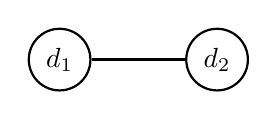
\begin{tikzpicture}[node distance=2cm, thick, main/.style = {draw, circle}]
        \node[main] (1) [] {$d_1$};
        \node[main] (2) [right of=1] {$d_2$};
        \draw[] (1) to (2);
    \end{tikzpicture}

}

\only<2>{
    \framesubtitle{Small-World effect (Triangles)}


    Set of three documents or concepts who are mutually connected, are a common feature of social networks and are thought to play an important role in social cohesion and network structure \citep{kossinets2006, newman2018}.

    \centering
    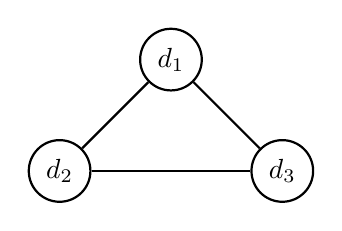
\begin{tikzpicture}[node distance=2cm, thick, main/.style = {draw, circle}]
        \node[main] (1) [] {$d_1$};
        \node[main] (2) [below left of=1] {$d_2$};
        \node[main] (3) [below right of=1] {$d_3$};
        \draw[] (1) to (2);
        \draw[] (1) to (3);
        \draw[] (2) to (3);
    \end{tikzpicture}
    % \caption{Closed Triad} 
    \label{fig:closed_triad}
}

\only<3>{
    \framesubtitle{Silo effect (Components)}

    \begin{itemize}

    \item Isolated areas of research or knowledge that are not well connected to other areas or fields 

    \item Limit the flow of information and influence within the network
    Hyper specialization of field of knowledge
    Talk to one another but never talk to nodes outside their primary group

    \end{itemize}

}

% \only<5>{
%     \framesubtitle{Closure effect (Transitivity)}

%     A triad is a group of three nodes in a graph. A triad can either be open or closed. An open triad is a group of three nodes that are connected by two edges (Figure \ref{fig:open_triad}), while a closed triad is a group of three nodes that are connected by three edges (Figure \ref{fig:closed_triad}). 

%     \begin{figure}[H]
%         \centering
%         \begin{subfigure}[t]{0.4\textwidth}
%             \centering
%             \begin{tikzpicture}[node distance=2cm, thick, main/.style = {draw, circle}]
%                 \node[main] (1) [] {$d_1$};
%                 \node[main] (2) [below left of=1] {$d_2$};
%                 \node[main] (3) [below right of=1] {$d_3$};
%                 \draw[] (1) to (2);
%                 \draw[] (1) to (3);
%             \end{tikzpicture}
%             \caption{Open Triad} 
%             \label{fig:open_triad}
%          \end{subfigure}
%             ~
%          \begin{subfigure}[t]{0.4\textwidth}
%             \centering
%             \begin{tikzpicture}[node distance=2cm, thick, main/.style = {draw, circle}]
%                 \node[main] (1) [] {$d_1$};
%                 \node[main] (2) [below left of=1] {$d_2$};
%                 \node[main] (3) [below right of=1] {$d_3$};
%                 \draw[] (1) to (2);
%                 \draw[] (1) to (3);
%                 \draw[] (2) to (3);
%             \end{tikzpicture}
%             \caption{Closed Triad} 
%             \label{fig:closed_triad}
%          \end{subfigure}
%          \caption{Triads}
%     \end{figure}

%     Transitivity is defined as the ratio of the number of closed triads in the graph to the number of open triads in the graph.

%     $$
%     T = \frac{3t_c}{t_o}
%     $$

%     Where $t_c$ is the number of closed triads and $t_o$ is the number of open triads.
% }

\only<4>{
    
    \framesubtitle{Clique effect (Cliques)}

    \begin{itemize}

        \item Set of fully connected nodes

        \item Represents subsets of documents or terms that are related closely to one another

        \item Distinct topical or functional units

    \end{itemize}

    % Tendecy for there to be parts of the graph where multiple nodes all co-occur more than by random change

    % If I discuss 
    % A all other concepts in the clique it belongs to.
    % highly related to each other distinct topical or functional units within the network

    % This build on triangles (which are a clique) but captures more information 

    % It asks whether triangles overlap to form larger structurees rather than just isolated (random) triangles

    % Densly connected always connected
}

\only<5>{
    \framesubtitle{Popularity effect ($k$-star)}

    % The popularity effects in most classes were not obvious, which meant the degree (the total number of actors selecting an individual) of individuals in the class networks had little difference.

    \begin{itemize}
        
        \item $k$ nodes connected to a central hub or a central node

        \item Measures tendency towards centralization 

    \end{itemize}

    \begin{figure}[H]
        \centering
        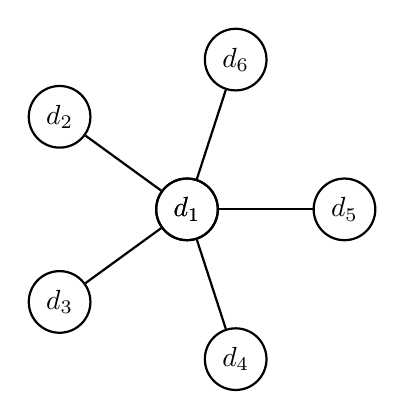
\begin{tikzpicture}[node distance=2cm, thick, main/.style = {draw, circle}]
            \node[main] (1) at (360:0mm) (center) {$d_1$};
            \node[main] (1) [] {$d_1$};
            \foreach \n in {2,...,6}{
                \node[main] at ({\n*360/5}:2cm) (n\n) {$d_\n$};
                \draw (center)--(n\n);
            }
        \end{tikzpicture}
        \caption{Star} \label{fig:k_star}
    \end{figure}

    % What we mean by a strong k star effect
    % Control for 9 stars in order to determine if 10 star is significant
    % 10 star is a bunch of 9 stars
}

% \only<8>{
%     \framesubtitle{Mediating effect (betweenness centrality)}

%     Nodes with high betweenness centrality in this type of network may represent important bridge terms or pivot terms that connect different topics or themes within the corpus of documents. The betweenness centrality $c_b$ of node $n$ is given by:

%     $$
%     c_b(i) = \sum_{j \ne k} \frac{\sigma_{jk}(i)}{\sigma_{jk}}
%     $$

%     Where $\sigma_{ij}$ is the total number of shortest paths from node $i$ to node $j$ and $\sigma_{ij}(n)$ is the number of those paths that pass through node $n$. In other words, it is the proportion of all shortest paths between nodes $i$ and $j$ that pass through node $n$. The average betweenness centrality over all nodes of the network is taken as another network statistic. 

%     Indicates good integration but maybe structural fragility (if central nodes are removed, speperate components)
% }

\only<6>{
    \framesubtitle{Community effect (Louvain)}

    \begin{itemize}
    
    \item Community detection algorithm
    
    \item Partition a network into distinct communities based on the structural patterns of connections between nodes

    \item Modularity maximization

    \end{itemize}

    % The Louvain community detection method consists of two main steps. Initially, each node is assigned to a separate community. Then, for each node, the algorithm attempts to optimize the modularity of the network by evaluating the potential gain in modularity achieved by moving the node to each of its neighboring communities. If no gain is achieved, the node remains in its original community.

    % In the second step, a new network is constructed where each node represents a community from the previous step. The edges between the new nodes are weighted by the sum of the weights of the edges between the nodes in the corresponding communities in the original network. The Louvain method is then applied to this new network, and the process is repeated until no further improvement in modularity can be achieved.

    % Modularity is a measure of the degree of segregation of a network into communities. It is calculated 
    % as the difference between the fraction of edges within a given group and the expected fraction of 
    % edges if they were randomly distributed in the network. The change in modularity $\Delta Q$ achieved 
    % by moving the node to each of its neighboring communities is measured as

    % $$
    % Q = \frac{1}{2m}\sum_{i,j}[A_{ij} - \frac{k_ik_j}{2m}]\delta(c_i,c_j)
    % $$

    % where:
    % \begin{itemize}
    %     \item $Q$ is the modularity index
    %     \item $m$ is the total number of edges in the network
    %     \item $A_{ij}$ is the weight of the edge between nodes $i$ and $j$
    %     \item $k_i$ and $k_j$ are the degrees of nodes $i$ and $j$, respectively
    %     \item $c_i$ and $c_j$ are the community assignments of nodes $i$ and $j$
    %     \item $\delta(c_i,c_j)$ is the Kronecker delta, which is equal to 1 if nodes $i$ and $j$ are in the same community and 0 otherwise.
    % \end{itemize}
}